% Created by tikzDevice version 0.12.3.1 on 2022-04-26 10:04:54
% !TEX encoding = UTF-8 Unicode
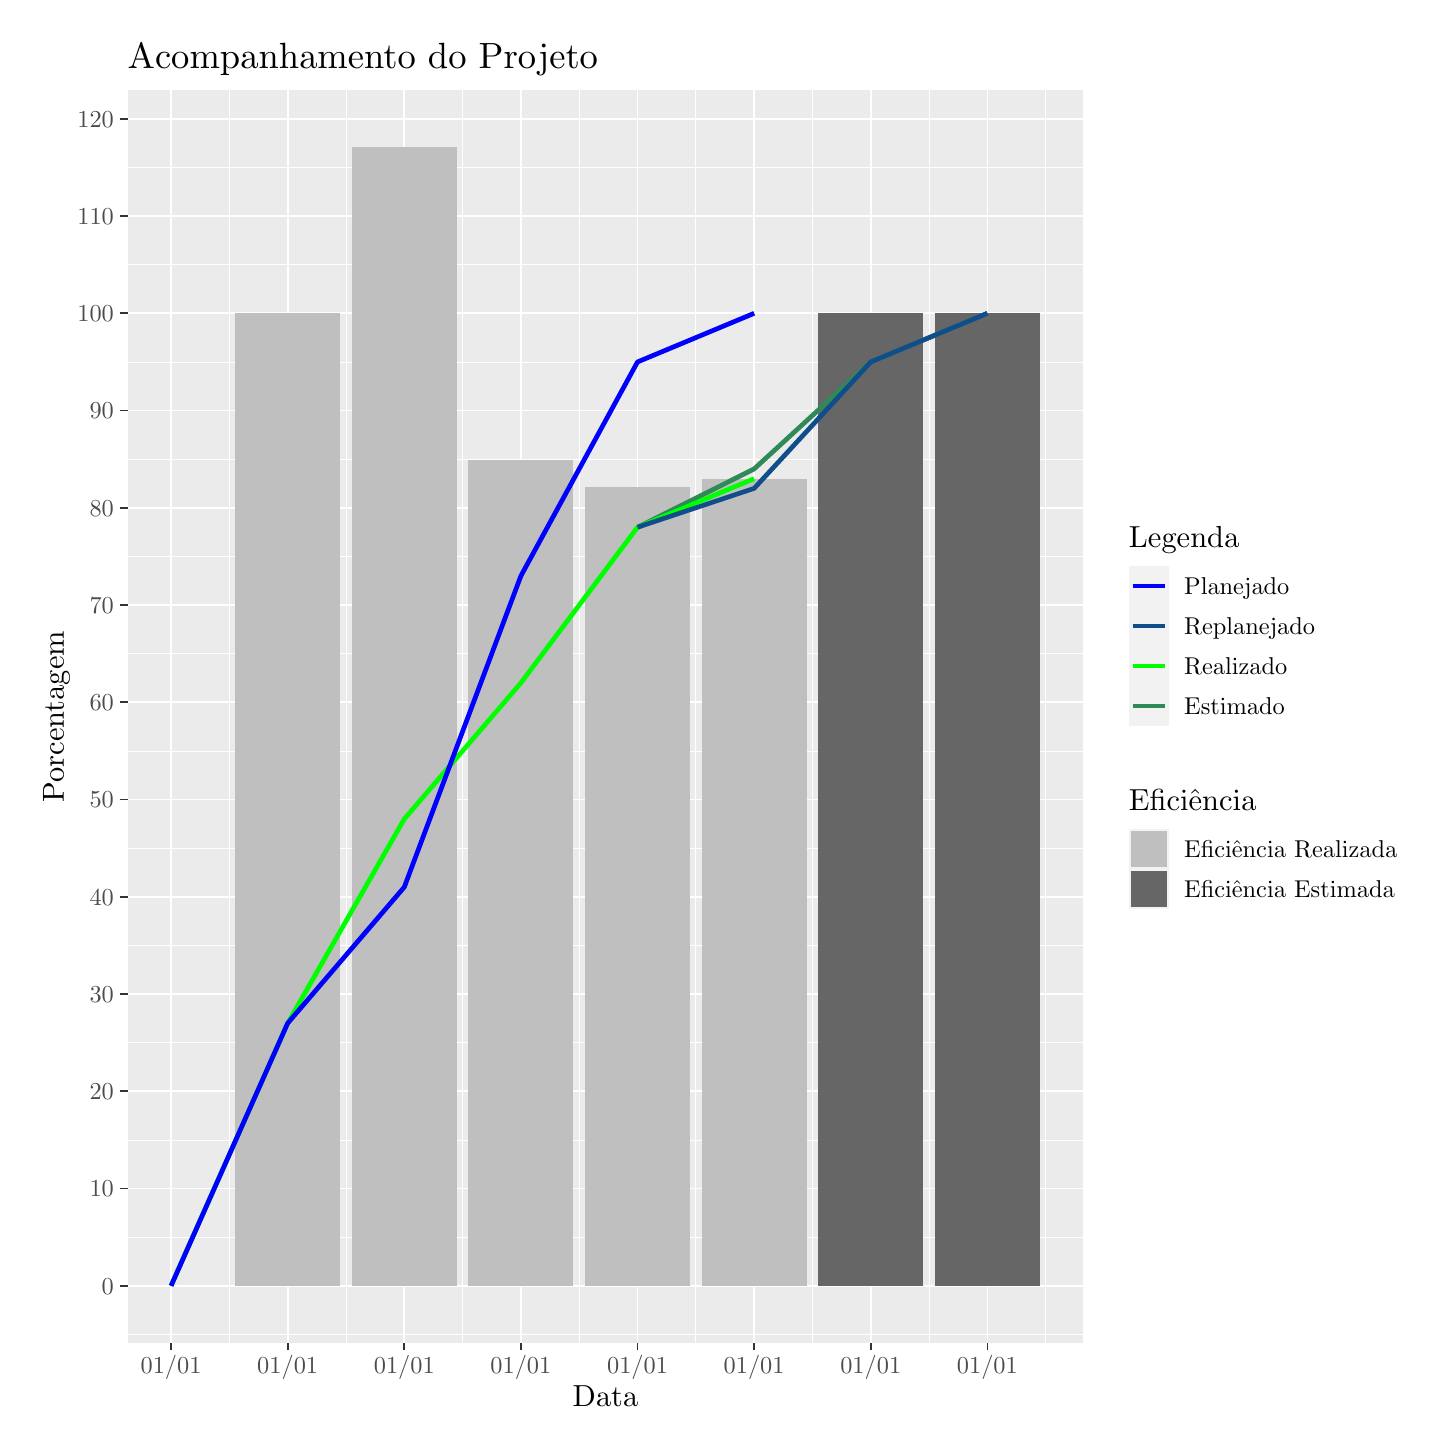
\begin{tikzpicture}[x=1pt,y=1pt]
\definecolor{fillColor}{RGB}{255,255,255}
\path[use as bounding box,fill=fillColor,fill opacity=0.00] (0,0) rectangle (505.89,505.89);
\begin{scope}
\path[clip] (  0.00,  0.00) rectangle (505.89,505.89);
\definecolor{drawColor}{RGB}{255,255,255}
\definecolor{fillColor}{RGB}{255,255,255}

\path[draw=drawColor,line width= 0.6pt,line join=round,line cap=round,fill=fillColor] (  0.00,  0.00) rectangle (505.89,505.89);
\end{scope}
\begin{scope}
\path[clip] ( 36.11, 30.69) rectangle (381.45,483.23);
\definecolor{fillColor}{gray}{0.92}

\path[fill=fillColor] ( 36.11, 30.69) rectangle (381.45,483.23);
\definecolor{drawColor}{RGB}{255,255,255}

\path[draw=drawColor,line width= 0.3pt,line join=round] ( 36.11, 33.69) --
	(381.45, 33.69);

\path[draw=drawColor,line width= 0.3pt,line join=round] ( 36.11, 68.83) --
	(381.45, 68.83);

\path[draw=drawColor,line width= 0.3pt,line join=round] ( 36.11,103.97) --
	(381.45,103.97);

\path[draw=drawColor,line width= 0.3pt,line join=round] ( 36.11,139.11) --
	(381.45,139.11);

\path[draw=drawColor,line width= 0.3pt,line join=round] ( 36.11,174.25) --
	(381.45,174.25);

\path[draw=drawColor,line width= 0.3pt,line join=round] ( 36.11,209.39) --
	(381.45,209.39);

\path[draw=drawColor,line width= 0.3pt,line join=round] ( 36.11,244.53) --
	(381.45,244.53);

\path[draw=drawColor,line width= 0.3pt,line join=round] ( 36.11,279.67) --
	(381.45,279.67);

\path[draw=drawColor,line width= 0.3pt,line join=round] ( 36.11,314.81) --
	(381.45,314.81);

\path[draw=drawColor,line width= 0.3pt,line join=round] ( 36.11,349.95) --
	(381.45,349.95);

\path[draw=drawColor,line width= 0.3pt,line join=round] ( 36.11,385.10) --
	(381.45,385.10);

\path[draw=drawColor,line width= 0.3pt,line join=round] ( 36.11,420.24) --
	(381.45,420.24);

\path[draw=drawColor,line width= 0.3pt,line join=round] ( 36.11,455.38) --
	(381.45,455.38);

\path[draw=drawColor,line width= 0.3pt,line join=round] ( 72.88, 30.69) --
	( 72.88,483.23);

\path[draw=drawColor,line width= 0.3pt,line join=round] (115.02, 30.69) --
	(115.02,483.23);

\path[draw=drawColor,line width= 0.3pt,line join=round] (157.16, 30.69) --
	(157.16,483.23);

\path[draw=drawColor,line width= 0.3pt,line join=round] (199.30, 30.69) --
	(199.30,483.23);

\path[draw=drawColor,line width= 0.3pt,line join=round] (241.44, 30.69) --
	(241.44,483.23);

\path[draw=drawColor,line width= 0.3pt,line join=round] (283.58, 30.69) --
	(283.58,483.23);

\path[draw=drawColor,line width= 0.3pt,line join=round] (325.72, 30.69) --
	(325.72,483.23);

\path[draw=drawColor,line width= 0.3pt,line join=round] (367.86, 30.69) --
	(367.86,483.23);

\path[draw=drawColor,line width= 0.6pt,line join=round] ( 36.11, 51.26) --
	(381.45, 51.26);

\path[draw=drawColor,line width= 0.6pt,line join=round] ( 36.11, 86.40) --
	(381.45, 86.40);

\path[draw=drawColor,line width= 0.6pt,line join=round] ( 36.11,121.54) --
	(381.45,121.54);

\path[draw=drawColor,line width= 0.6pt,line join=round] ( 36.11,156.68) --
	(381.45,156.68);

\path[draw=drawColor,line width= 0.6pt,line join=round] ( 36.11,191.82) --
	(381.45,191.82);

\path[draw=drawColor,line width= 0.6pt,line join=round] ( 36.11,226.96) --
	(381.45,226.96);

\path[draw=drawColor,line width= 0.6pt,line join=round] ( 36.11,262.10) --
	(381.45,262.10);

\path[draw=drawColor,line width= 0.6pt,line join=round] ( 36.11,297.24) --
	(381.45,297.24);

\path[draw=drawColor,line width= 0.6pt,line join=round] ( 36.11,332.38) --
	(381.45,332.38);

\path[draw=drawColor,line width= 0.6pt,line join=round] ( 36.11,367.52) --
	(381.45,367.52);

\path[draw=drawColor,line width= 0.6pt,line join=round] ( 36.11,402.67) --
	(381.45,402.67);

\path[draw=drawColor,line width= 0.6pt,line join=round] ( 36.11,437.81) --
	(381.45,437.81);

\path[draw=drawColor,line width= 0.6pt,line join=round] ( 36.11,472.95) --
	(381.45,472.95);

\path[draw=drawColor,line width= 0.6pt,line join=round] ( 51.81, 30.69) --
	( 51.81,483.23);

\path[draw=drawColor,line width= 0.6pt,line join=round] ( 93.95, 30.69) --
	( 93.95,483.23);

\path[draw=drawColor,line width= 0.6pt,line join=round] (136.09, 30.69) --
	(136.09,483.23);

\path[draw=drawColor,line width= 0.6pt,line join=round] (178.23, 30.69) --
	(178.23,483.23);

\path[draw=drawColor,line width= 0.6pt,line join=round] (220.37, 30.69) --
	(220.37,483.23);

\path[draw=drawColor,line width= 0.6pt,line join=round] (262.51, 30.69) --
	(262.51,483.23);

\path[draw=drawColor,line width= 0.6pt,line join=round] (304.65, 30.69) --
	(304.65,483.23);

\path[draw=drawColor,line width= 0.6pt,line join=round] (346.79, 30.69) --
	(346.79,483.23);
\definecolor{fillColor}{gray}{0.75}

\path[fill=fillColor] ( 74.99, 51.26) rectangle (112.91,402.67);

\path[fill=fillColor] (117.13, 51.26) rectangle (155.05,462.66);

\path[fill=fillColor] (159.27, 51.26) rectangle (197.19,349.71);

\path[fill=fillColor] (201.41, 51.26) rectangle (239.33,339.78);

\path[fill=fillColor] (243.55, 51.26) rectangle (281.48,342.93);
\definecolor{fillColor}{gray}{0.40}

\path[fill=fillColor] (285.69, 51.26) rectangle (323.62,402.67);

\path[fill=fillColor] (327.83, 51.26) rectangle (365.76,402.67);
\definecolor{drawColor}{RGB}{46,139,87}

\path[draw=drawColor,line width= 1.7pt,line join=round] (220.37,325.36) --
	(262.51,346.44) --
	(304.65,385.10) --
	(346.79,402.67);
\definecolor{drawColor}{RGB}{0,255,0}

\path[draw=drawColor,line width= 1.7pt,line join=round] ( 51.81, 51.26) --
	( 93.95,146.14) --
	(136.09,219.93) --
	(178.23,269.13) --
	(220.37,325.36) --
	(262.51,342.93);
\definecolor{drawColor}{RGB}{0,0,255}

\path[draw=drawColor,line width= 1.7pt,line join=round] ( 51.81, 51.26) --
	( 93.95,146.14) --
	(136.09,195.33) --
	(178.23,307.79) --
	(220.37,385.10) --
	(262.51,402.67);
\definecolor{drawColor}{RGB}{16,78,139}

\path[draw=drawColor,line width= 1.7pt,line join=round] (220.37,325.36) --
	(262.51,339.41) --
	(304.65,385.10) --
	(346.79,402.67);
\end{scope}
\begin{scope}
\path[clip] (  0.00,  0.00) rectangle (505.89,505.89);
\definecolor{drawColor}{gray}{0.30}

\node[text=drawColor,anchor=base east,inner sep=0pt, outer sep=0pt, scale=  0.88] at ( 31.16, 48.23) {0};

\node[text=drawColor,anchor=base east,inner sep=0pt, outer sep=0pt, scale=  0.88] at ( 31.16, 83.37) {10};

\node[text=drawColor,anchor=base east,inner sep=0pt, outer sep=0pt, scale=  0.88] at ( 31.16,118.51) {20};

\node[text=drawColor,anchor=base east,inner sep=0pt, outer sep=0pt, scale=  0.88] at ( 31.16,153.65) {30};

\node[text=drawColor,anchor=base east,inner sep=0pt, outer sep=0pt, scale=  0.88] at ( 31.16,188.79) {40};

\node[text=drawColor,anchor=base east,inner sep=0pt, outer sep=0pt, scale=  0.88] at ( 31.16,223.93) {50};

\node[text=drawColor,anchor=base east,inner sep=0pt, outer sep=0pt, scale=  0.88] at ( 31.16,259.07) {60};

\node[text=drawColor,anchor=base east,inner sep=0pt, outer sep=0pt, scale=  0.88] at ( 31.16,294.21) {70};

\node[text=drawColor,anchor=base east,inner sep=0pt, outer sep=0pt, scale=  0.88] at ( 31.16,329.35) {80};

\node[text=drawColor,anchor=base east,inner sep=0pt, outer sep=0pt, scale=  0.88] at ( 31.16,364.49) {90};

\node[text=drawColor,anchor=base east,inner sep=0pt, outer sep=0pt, scale=  0.88] at ( 31.16,399.64) {100};

\node[text=drawColor,anchor=base east,inner sep=0pt, outer sep=0pt, scale=  0.88] at ( 31.16,434.78) {110};

\node[text=drawColor,anchor=base east,inner sep=0pt, outer sep=0pt, scale=  0.88] at ( 31.16,469.92) {120};
\end{scope}
\begin{scope}
\path[clip] (  0.00,  0.00) rectangle (505.89,505.89);
\definecolor{drawColor}{gray}{0.20}

\path[draw=drawColor,line width= 0.6pt,line join=round] ( 33.36, 51.26) --
	( 36.11, 51.26);

\path[draw=drawColor,line width= 0.6pt,line join=round] ( 33.36, 86.40) --
	( 36.11, 86.40);

\path[draw=drawColor,line width= 0.6pt,line join=round] ( 33.36,121.54) --
	( 36.11,121.54);

\path[draw=drawColor,line width= 0.6pt,line join=round] ( 33.36,156.68) --
	( 36.11,156.68);

\path[draw=drawColor,line width= 0.6pt,line join=round] ( 33.36,191.82) --
	( 36.11,191.82);

\path[draw=drawColor,line width= 0.6pt,line join=round] ( 33.36,226.96) --
	( 36.11,226.96);

\path[draw=drawColor,line width= 0.6pt,line join=round] ( 33.36,262.10) --
	( 36.11,262.10);

\path[draw=drawColor,line width= 0.6pt,line join=round] ( 33.36,297.24) --
	( 36.11,297.24);

\path[draw=drawColor,line width= 0.6pt,line join=round] ( 33.36,332.38) --
	( 36.11,332.38);

\path[draw=drawColor,line width= 0.6pt,line join=round] ( 33.36,367.52) --
	( 36.11,367.52);

\path[draw=drawColor,line width= 0.6pt,line join=round] ( 33.36,402.67) --
	( 36.11,402.67);

\path[draw=drawColor,line width= 0.6pt,line join=round] ( 33.36,437.81) --
	( 36.11,437.81);

\path[draw=drawColor,line width= 0.6pt,line join=round] ( 33.36,472.95) --
	( 36.11,472.95);
\end{scope}
\begin{scope}
\path[clip] (  0.00,  0.00) rectangle (505.89,505.89);
\definecolor{drawColor}{gray}{0.20}

\path[draw=drawColor,line width= 0.6pt,line join=round] ( 51.81, 27.94) --
	( 51.81, 30.69);

\path[draw=drawColor,line width= 0.6pt,line join=round] ( 93.95, 27.94) --
	( 93.95, 30.69);

\path[draw=drawColor,line width= 0.6pt,line join=round] (136.09, 27.94) --
	(136.09, 30.69);

\path[draw=drawColor,line width= 0.6pt,line join=round] (178.23, 27.94) --
	(178.23, 30.69);

\path[draw=drawColor,line width= 0.6pt,line join=round] (220.37, 27.94) --
	(220.37, 30.69);

\path[draw=drawColor,line width= 0.6pt,line join=round] (262.51, 27.94) --
	(262.51, 30.69);

\path[draw=drawColor,line width= 0.6pt,line join=round] (304.65, 27.94) --
	(304.65, 30.69);

\path[draw=drawColor,line width= 0.6pt,line join=round] (346.79, 27.94) --
	(346.79, 30.69);
\end{scope}
\begin{scope}
\path[clip] (  0.00,  0.00) rectangle (505.89,505.89);
\definecolor{drawColor}{gray}{0.30}

\node[text=drawColor,anchor=base,inner sep=0pt, outer sep=0pt, scale=  0.88] at ( 51.81, 19.68) {01/01};

\node[text=drawColor,anchor=base,inner sep=0pt, outer sep=0pt, scale=  0.88] at ( 93.95, 19.68) {01/01};

\node[text=drawColor,anchor=base,inner sep=0pt, outer sep=0pt, scale=  0.88] at (136.09, 19.68) {01/01};

\node[text=drawColor,anchor=base,inner sep=0pt, outer sep=0pt, scale=  0.88] at (178.23, 19.68) {01/01};

\node[text=drawColor,anchor=base,inner sep=0pt, outer sep=0pt, scale=  0.88] at (220.37, 19.68) {01/01};

\node[text=drawColor,anchor=base,inner sep=0pt, outer sep=0pt, scale=  0.88] at (262.51, 19.68) {01/01};

\node[text=drawColor,anchor=base,inner sep=0pt, outer sep=0pt, scale=  0.88] at (304.65, 19.68) {01/01};

\node[text=drawColor,anchor=base,inner sep=0pt, outer sep=0pt, scale=  0.88] at (346.79, 19.68) {01/01};
\end{scope}
\begin{scope}
\path[clip] (  0.00,  0.00) rectangle (505.89,505.89);
\definecolor{drawColor}{RGB}{0,0,0}

\node[text=drawColor,anchor=base,inner sep=0pt, outer sep=0pt, scale=  1.10] at (208.78,  7.64) {Data};
\end{scope}
\begin{scope}
\path[clip] (  0.00,  0.00) rectangle (505.89,505.89);
\definecolor{drawColor}{RGB}{0,0,0}

\node[text=drawColor,rotate= 90.00,anchor=base,inner sep=0pt, outer sep=0pt, scale=  1.10] at ( 13.08,256.96) {Porcentagem};
\end{scope}
\begin{scope}
\path[clip] (  0.00,  0.00) rectangle (505.89,505.89);
\definecolor{fillColor}{RGB}{255,255,255}

\path[fill=fillColor] (392.45,248.01) rectangle (470.70,332.04);
\end{scope}
\begin{scope}
\path[clip] (  0.00,  0.00) rectangle (505.89,505.89);
\definecolor{drawColor}{RGB}{0,0,0}

\node[text=drawColor,anchor=base west,inner sep=0pt, outer sep=0pt, scale=  1.10] at (397.95,317.89) {Legenda};
\end{scope}
\begin{scope}
\path[clip] (  0.00,  0.00) rectangle (505.89,505.89);
\definecolor{fillColor}{gray}{0.95}

\path[fill=fillColor] (397.95,296.87) rectangle (412.41,311.32);
\end{scope}
\begin{scope}
\path[clip] (  0.00,  0.00) rectangle (505.89,505.89);
\definecolor{drawColor}{RGB}{0,0,255}

\path[draw=drawColor,line width= 1.7pt,line join=round] (399.40,304.09) -- (410.96,304.09);
\end{scope}
\begin{scope}
\path[clip] (  0.00,  0.00) rectangle (505.89,505.89);
\definecolor{drawColor}{RGB}{0,0,255}

\path[draw=drawColor,line width= 1.7pt,line join=round] (399.40,304.09) -- (410.96,304.09);
\end{scope}
\begin{scope}
\path[clip] (  0.00,  0.00) rectangle (505.89,505.89);
\definecolor{drawColor}{RGB}{0,0,255}

\path[draw=drawColor,line width= 1.7pt,line join=round] (399.40,304.09) -- (410.96,304.09);
\end{scope}
\begin{scope}
\path[clip] (  0.00,  0.00) rectangle (505.89,505.89);
\definecolor{drawColor}{RGB}{0,0,255}

\path[draw=drawColor,line width= 1.7pt,line join=round] (399.40,304.09) -- (410.96,304.09);
\end{scope}
\begin{scope}
\path[clip] (  0.00,  0.00) rectangle (505.89,505.89);
\definecolor{fillColor}{gray}{0.95}

\path[fill=fillColor] (397.95,282.41) rectangle (412.41,296.87);
\end{scope}
\begin{scope}
\path[clip] (  0.00,  0.00) rectangle (505.89,505.89);
\definecolor{drawColor}{RGB}{16,78,139}

\path[draw=drawColor,line width= 1.7pt,line join=round] (399.40,289.64) -- (410.96,289.64);
\end{scope}
\begin{scope}
\path[clip] (  0.00,  0.00) rectangle (505.89,505.89);
\definecolor{drawColor}{RGB}{16,78,139}

\path[draw=drawColor,line width= 1.7pt,line join=round] (399.40,289.64) -- (410.96,289.64);
\end{scope}
\begin{scope}
\path[clip] (  0.00,  0.00) rectangle (505.89,505.89);
\definecolor{drawColor}{RGB}{16,78,139}

\path[draw=drawColor,line width= 1.7pt,line join=round] (399.40,289.64) -- (410.96,289.64);
\end{scope}
\begin{scope}
\path[clip] (  0.00,  0.00) rectangle (505.89,505.89);
\definecolor{drawColor}{RGB}{16,78,139}

\path[draw=drawColor,line width= 1.7pt,line join=round] (399.40,289.64) -- (410.96,289.64);
\end{scope}
\begin{scope}
\path[clip] (  0.00,  0.00) rectangle (505.89,505.89);
\definecolor{fillColor}{gray}{0.95}

\path[fill=fillColor] (397.95,267.96) rectangle (412.41,282.41);
\end{scope}
\begin{scope}
\path[clip] (  0.00,  0.00) rectangle (505.89,505.89);
\definecolor{drawColor}{RGB}{0,255,0}

\path[draw=drawColor,line width= 1.7pt,line join=round] (399.40,275.19) -- (410.96,275.19);
\end{scope}
\begin{scope}
\path[clip] (  0.00,  0.00) rectangle (505.89,505.89);
\definecolor{drawColor}{RGB}{0,255,0}

\path[draw=drawColor,line width= 1.7pt,line join=round] (399.40,275.19) -- (410.96,275.19);
\end{scope}
\begin{scope}
\path[clip] (  0.00,  0.00) rectangle (505.89,505.89);
\definecolor{drawColor}{RGB}{0,255,0}

\path[draw=drawColor,line width= 1.7pt,line join=round] (399.40,275.19) -- (410.96,275.19);
\end{scope}
\begin{scope}
\path[clip] (  0.00,  0.00) rectangle (505.89,505.89);
\definecolor{drawColor}{RGB}{0,255,0}

\path[draw=drawColor,line width= 1.7pt,line join=round] (399.40,275.19) -- (410.96,275.19);
\end{scope}
\begin{scope}
\path[clip] (  0.00,  0.00) rectangle (505.89,505.89);
\definecolor{fillColor}{gray}{0.95}

\path[fill=fillColor] (397.95,253.51) rectangle (412.41,267.96);
\end{scope}
\begin{scope}
\path[clip] (  0.00,  0.00) rectangle (505.89,505.89);
\definecolor{drawColor}{RGB}{46,139,87}

\path[draw=drawColor,line width= 1.7pt,line join=round] (399.40,260.73) -- (410.96,260.73);
\end{scope}
\begin{scope}
\path[clip] (  0.00,  0.00) rectangle (505.89,505.89);
\definecolor{drawColor}{RGB}{46,139,87}

\path[draw=drawColor,line width= 1.7pt,line join=round] (399.40,260.73) -- (410.96,260.73);
\end{scope}
\begin{scope}
\path[clip] (  0.00,  0.00) rectangle (505.89,505.89);
\definecolor{drawColor}{RGB}{46,139,87}

\path[draw=drawColor,line width= 1.7pt,line join=round] (399.40,260.73) -- (410.96,260.73);
\end{scope}
\begin{scope}
\path[clip] (  0.00,  0.00) rectangle (505.89,505.89);
\definecolor{drawColor}{RGB}{46,139,87}

\path[draw=drawColor,line width= 1.7pt,line join=round] (399.40,260.73) -- (410.96,260.73);
\end{scope}
\begin{scope}
\path[clip] (  0.00,  0.00) rectangle (505.89,505.89);
\definecolor{drawColor}{RGB}{0,0,0}

\node[text=drawColor,anchor=base west,inner sep=0pt, outer sep=0pt, scale=  0.88] at (417.91,301.06) {Planejado};
\end{scope}
\begin{scope}
\path[clip] (  0.00,  0.00) rectangle (505.89,505.89);
\definecolor{drawColor}{RGB}{0,0,0}

\node[text=drawColor,anchor=base west,inner sep=0pt, outer sep=0pt, scale=  0.88] at (417.91,286.61) {Replanejado};
\end{scope}
\begin{scope}
\path[clip] (  0.00,  0.00) rectangle (505.89,505.89);
\definecolor{drawColor}{RGB}{0,0,0}

\node[text=drawColor,anchor=base west,inner sep=0pt, outer sep=0pt, scale=  0.88] at (417.91,272.16) {Realizado};
\end{scope}
\begin{scope}
\path[clip] (  0.00,  0.00) rectangle (505.89,505.89);
\definecolor{drawColor}{RGB}{0,0,0}

\node[text=drawColor,anchor=base west,inner sep=0pt, outer sep=0pt, scale=  0.88] at (417.91,257.70) {Estimado};
\end{scope}
\begin{scope}
\path[clip] (  0.00,  0.00) rectangle (505.89,505.89);
\definecolor{fillColor}{RGB}{255,255,255}

\path[fill=fillColor] (392.45,181.88) rectangle (500.39,237.01);
\end{scope}
\begin{scope}
\path[clip] (  0.00,  0.00) rectangle (505.89,505.89);
\definecolor{drawColor}{RGB}{0,0,0}

\node[text=drawColor,anchor=base west,inner sep=0pt, outer sep=0pt, scale=  1.10] at (397.95,222.86) {Eficiência};
\end{scope}
\begin{scope}
\path[clip] (  0.00,  0.00) rectangle (505.89,505.89);
\definecolor{fillColor}{gray}{0.95}

\path[fill=fillColor] (397.95,201.84) rectangle (412.41,216.29);
\end{scope}
\begin{scope}
\path[clip] (  0.00,  0.00) rectangle (505.89,505.89);
\definecolor{fillColor}{gray}{0.75}

\path[fill=fillColor] (398.67,202.55) rectangle (411.70,215.58);
\end{scope}
\begin{scope}
\path[clip] (  0.00,  0.00) rectangle (505.89,505.89);
\definecolor{fillColor}{gray}{0.75}

\path[fill=fillColor] (398.67,202.55) rectangle (411.70,215.58);
\end{scope}
\begin{scope}
\path[clip] (  0.00,  0.00) rectangle (505.89,505.89);
\definecolor{fillColor}{gray}{0.95}

\path[fill=fillColor] (397.95,187.38) rectangle (412.41,201.84);
\end{scope}
\begin{scope}
\path[clip] (  0.00,  0.00) rectangle (505.89,505.89);
\definecolor{fillColor}{gray}{0.40}

\path[fill=fillColor] (398.67,188.09) rectangle (411.70,201.13);
\end{scope}
\begin{scope}
\path[clip] (  0.00,  0.00) rectangle (505.89,505.89);
\definecolor{fillColor}{gray}{0.40}

\path[fill=fillColor] (398.67,188.09) rectangle (411.70,201.13);
\end{scope}
\begin{scope}
\path[clip] (  0.00,  0.00) rectangle (505.89,505.89);
\definecolor{drawColor}{RGB}{0,0,0}

\node[text=drawColor,anchor=base west,inner sep=0pt, outer sep=0pt, scale=  0.88] at (417.91,206.03) {Eficiência Realizada};
\end{scope}
\begin{scope}
\path[clip] (  0.00,  0.00) rectangle (505.89,505.89);
\definecolor{drawColor}{RGB}{0,0,0}

\node[text=drawColor,anchor=base west,inner sep=0pt, outer sep=0pt, scale=  0.88] at (417.91,191.58) {Eficiência Estimada};
\end{scope}
\begin{scope}
\path[clip] (  0.00,  0.00) rectangle (505.89,505.89);
\definecolor{drawColor}{RGB}{0,0,0}

\node[text=drawColor,anchor=base west,inner sep=0pt, outer sep=0pt, scale=  1.32] at ( 36.11,491.30) {Acompanhamento do Projeto};
\end{scope}
\end{tikzpicture}
